\section{Method}
\label{sec:method}
In this section, we will first define our task and weighted decoding method for controllable generation as background. Then we will introduce the proposed \textbf{DASC} framework. 
\subsection{Task Definition}

Given a dialogue \textbf{context} $C$ and \textbf{attributes} $A = (a_1, a_2, ..., a_K)$, \textit{Controllable Dialogue Generation} aims to generate a \textbf{response} $R = (r_1, r_2, ..., r_N)$ that is consistent with the context 
and carries the attributes.\footnote{In our work, we make a pre-assumption that attributes 
are provided by a dialogue policy, and do not include end-to-end scenarios.}
There can be multiple \textbf{aspects} grouping the attributes, where in this work we will focus on \textit{Gender Style, Emotion, and Dialogue Act}. An aspect covers multiple related attributes, such as \textit{happiness, sadness} for the Emotion aspect. Each attribute can take three values: 1 means to use the attribute, 0 means not to use and $\phi$ means the attribute is not
applicable to the response.

\subsection{Weighted Decoding for Controllable Generation}
\label{sec:weighted_decoding}

Standard, non-controllable, dialogue generation can be formulated with the standard conditional language modeling objective: $L_{CLM} = -\sum_{n=1}^N log P(r_n|r_{1:n-1}, C)$

We can use a transformer-based encoder-decoder architecture like BART \cite{lewis2020bart} to model this, where the encoder encodes the context into hidden states as condition for the decoder to generate the response. We will omit $C$ below for brevity.

In controllable dialogue generation, we additionally introduce attributes in the generation condition. Suppose we are generating with a single attribute $a$, then the objective is to model $P(r_n|r_{1:n-1}, a)$. Using Bayes' rule, this can be converted to:
% \KZ{It's not good to use small font for equations. Note that the equation
% numbers have also been shrunk and inconsistent across the paper (some big,
% some small).}
\begin{equation}
    \small
    P(r_n|r_{1:n-1}, a) \propto P(r_n|r_{1:n-1}) P(a|r_{1:n-1}, r_n)^{\alpha}
    \label{eqn:single_wd}
\end{equation}
where $\alpha$ is a hyperparameter that can adjust the \textit{control strength}. This means that we can decompose the generation probability into the standard CLM probability weighted by the prediction of another token-wise attribute classifier during decoding. Methods established on such decomposition are thus called \textbf{Weighted Decoding} models.

Director \citep{arora2022director}, a representative weighted decoding method, implements the attribute classifier as a linear layer on top of the decoder hidden states. A binary classification is performed on determining whether the generated sentence reflects the desired attribute (e.g. happy or not) at each step. For tokens in the sentence from training set, they can be trained with the attribute of the whole sentence using Binary Cross Entropy (BCE) loss. We denote this token-level loss as $L_{t}$. 

\begin{equation}
    \begin{aligned}
        L_{t} &= BCE(P(a | r_{1:n-1}, r_n)) \\
                  &= BCE(\sigma([W_a h_n]_{r_n}))
    \end{aligned}
    \label{eqn:clf_t}
\end{equation}
where $h_n \in \mathbb{R}^{d}$ is the hidden state for the $n$-th token, $W_a \in \mathbb{R}^{|V| \times d}$ is the learnable weight matrix for attribute prediction given the generation of each token in the vocabulary, and $[\cdot]_{r_n}$ denotes the index selection with the next token $r_n$. 
Note that it only gathers the attribute logits with the token $r_n$ 
in the ground truth response. For the other $|V|-1$ tokens in the vocabulary 
$V$, they have no label and cannot get trained. Therefore, it uses an 
extra regularizer to train the prediction on these tokens to as close to 
0.5 as possible with MSE loss.  

When dealing with multi-attribute control, we can extend 
\eqnref{eqn:single_wd} by introducing the product of multiple attribute 
classifiers, assuming the conditional independence of attributes:

\begin{equation}
    \small
    P(r_n|r_{1:n-1}, a) \propto P(r_n|r_{1:n-1}) \prod_{\substack{k=1\\a_k\ne \phi}}^{K} P(a_k|r_{1:n})^{\alpha}
    \label{eqn:multi_wd}
\end{equation}

The product of probabilities is usually implemented with the 
summation of logits: 
% \KZ{Logistic function is usually $\sigma$, not $\delta$?} 
% \ZL{I'm not using it to stand for logistic function, but the logits before the softmax/logistic function to get probabilities.}

\begin{equation}
    \small
    \delta(r_n|r_{1:n-1}, a) = \delta(r_n|r_{1:n-1}) + \alpha \sum_{\substack{k=1\\a_k\ne \phi}}^{K} \delta(a_k|r_{1:n})
    \label{eqn:multi_wd_logits}
\end{equation}

Existing works have implemented such an extension with either multiple forward passes through an 
attribute-conditioned language model \citep{lin2021plug} or one pass 
of multiple models \citep{liu2021dexperts}, which can all be very costly as the number of attributes grows. 
Here we introduce a relatively simple extension of Director, where we just add $K$ linear classifier heads to 
make the prediction of multiple attributes. We will refer to this 
simple extension as M-Director, or just Director for simplicity.
Note that though more efficient than previous methods, M-Director will still introduce $d \times |V| \times K$ extra parameters.
Given that $|V|$ is usually as large as tens of thousands, this model will 
have enormous number of parameters making it inefficient to train or infer, 
and also prone to overfitting. 

\subsection{Dialogue Attribute Space Controller}
\label{sec:dasc_method}
We hypothesize that the above typical methods of weighted decoding may 
not be the most efficient approach to learn the token-level attribute 
semantics, especially in multi-attribute cases. 
The learning objective is imposed on a single token in the target sentence, 
while all  other tokens are regularized equally. This is not usually reasonable, as some tokens similar to the target token should also have high probabilities 
given the attribute while other tokens different from it are less likely to be 
generated. For example, for the first token in a \textit{happy} response ``nice to meet you'', ``glad'' will also be a reasonable alternative, 
while ``sad'' is not, but their attribute label in the training will both 
be 0.5.

We can fix this counter-intuition in a high-dimensional space. 
On the one hand, each token has an $p$-dim embedding that encodes its attribute 
semantics (\textit{Attribute Token Embedding}, $ATEMB$). 
On the other hand, the hidden states from the LM ($h_n$) are also projected 
to the same space with attribute-specific linear layers 
($W^k \in \mathbb{R}^{p \times d}$) to get 
\textit{Attribute Context Embedding}, $\hat h^k_n = \hat W^k h_n$.
Thus different vectors in the space convey different semantics, 
and we call this space \textit{Attribute Semantic Space}. 

To leverage this latent space for weighted decoding, for each $\hat h^k_n$, we find its attribute-related tokens according to embedding similarity in the space, and assign them higher weights during decoding. Specifically, it is accomplished with a dot-product based token-level attribute classifier.


\begin{equation}
    \small
    \delta(a_k|r_{1:n}) = \hat h^k_n \cdot ATEMB(r_n)
    \label{eqn:matching_for_logits}
\end{equation}

In this case, when a token is trained with high probability for 
certain attribute, its neighbors in the attribute space will also 
have higher probabilities. This alleviates the limitation of previous 
weighted decoding methods, and eliminates the need for regularizers on 
other tokens. Further, when applying this to multi-attribute weighted decoding, 
we get: 

\begin{equation}
    \small
    \begin{aligned}
        \delta(r_n|r_{1:n-1}, a) &= \delta(r_n|r_{1:n-1}) \\
                                 &+ \alpha (\frac{1}{K} \sum_{\substack{k=1\\a_k\ne \phi}}^{K} \hat h^k_n) \cdot ATEMB(r_n)
    \end{aligned}
    \label{eqn:dasc_logits}
\end{equation}
where the parenthesized part in the second term can be interpreted as the 
average/equal-weight interpolation of multiple attribute context embeddings.
% \KZ{Why multiply by K? Doesn't this cancel out the K on the denominator?} 
% \ZL{Make it more close to interpolation in the forumulation}
\footnote{It is possible to assign different weights for each embedding in interpolation, and we leave it for future works.}
This formulation suggests that if the attribute space is properly learned and represented, the embedding interpolation will precisely reflect the semantics of the desired attributes, and then DASC can realize reasonable attribute combinations. 

\begin{figure}[t]
    \centering
    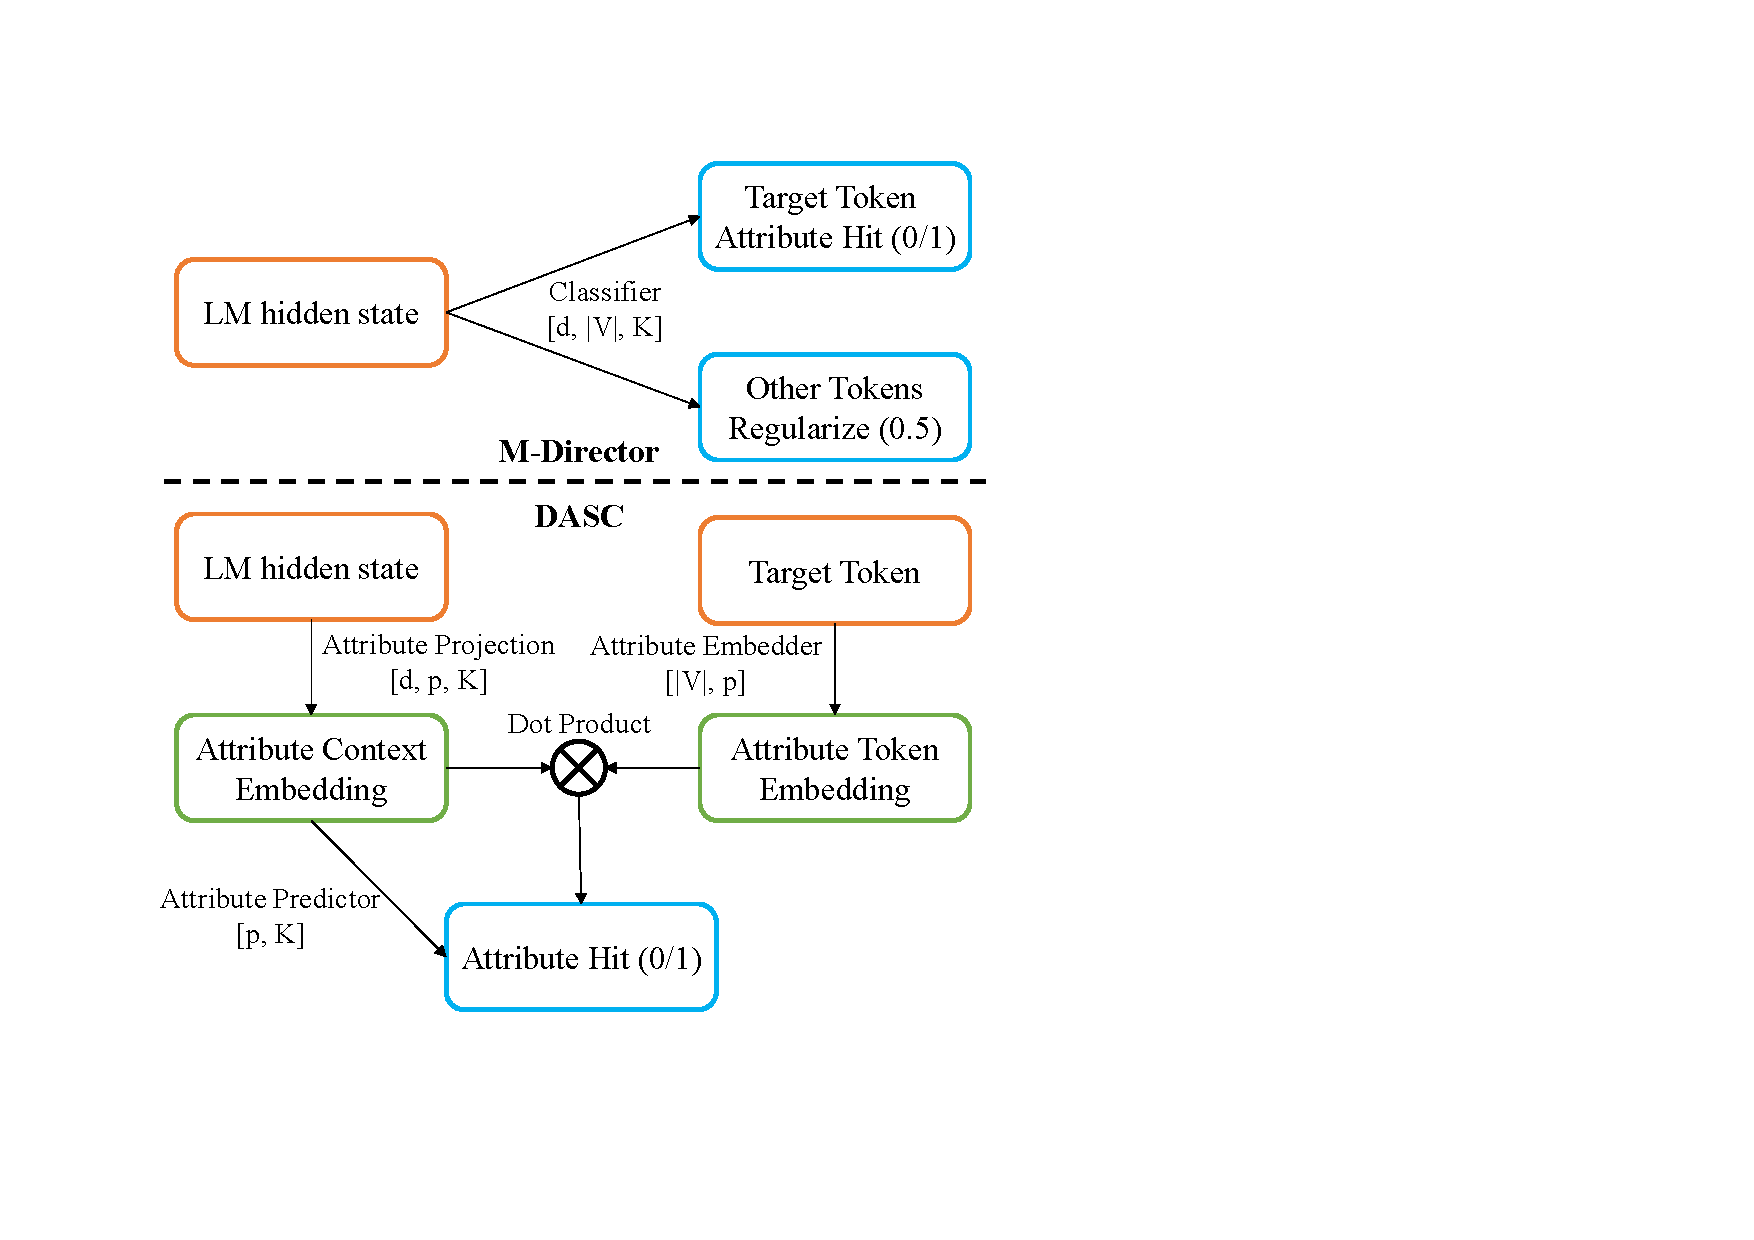
\includegraphics[width=1.0\columnwidth]{figures/dasc_illustration.pdf}
    \caption{Framework comparison between M-Director and DASC. M-Director uses a classifier head to conduct binary attribute hit classification for each token in the target sentence, and impose regularization for other tokens. 
DASC projects both LM hidden state and the target token to the attribute space, and uses their dot product for the classification of attribute hit. 
For each parameterized model component, we show its shape in square brackets.}
    \label{fig:dasc_illustration}
\end{figure}

To assist the learning of attribute embeddings, we introduce another linear layer on top of the attribute context embedding at each step to directly predict the attributes of the complete response. This can help better align the attribute 
context embeddings with the corresponding region for its attributes. 
We denote the new the sentence-level classification loss as $L_{s}$. 
For clarity, we give its formulation in the single-attribute case, 
which can be simply extended to multi-attribute scenarios with the 
summation over all non-empty attributes.

\begin{equation}
    \begin{aligned}
        L_{s} &= BCE(P(a | r_{1:n-1})) \\
                  &= BCE(\sigma(v_a \cdot \hat h_n))
    \end{aligned}
\end{equation}
where $v_a \in \mathbb{R}^{p}$ is the learnable weight for attribute prediction. Compared with $L_{t}$ (\eqnref{eqn:clf_t}), it is a sentence-level classification task independent of $r_n$, which can also be interpreted as predicting the prior probability of the attribute before deciding the next token to generate, and thus the parameters do not scale with $|V|$. Then the final loss is: $L_{train} = L_{CLM} + \beta (L_{s} + L_{t})$, where $\beta$ is a hyperparameter that controls the weight of attribute-related losses.

We name the proposed framework as Dialogue Attribute Space Controller (\textbf{DASC}). The illustration of DASC and its comparison with M-Director is shown in Figure \ref{fig:dasc_illustration}. DASC introduce fewer parameters ($d\times p \times K + |V| \times p$)  than M-Director ($d \times |V| \times K$). Since we set $p << |V|$, the parameters of attributes projections will be much smaller. And when we deal with $K > 1$, the shared token embeddings across attributes will also save parameters, while the parameters of attribute predictor are almost negligible. % As we will validate in Sec. \ref{sec:parameter_analysis}, the suitable amount of parameters also helps DASC achieve a better balance between controllability and generation quality. 
% \MY{This balance between controllability and quality can be made more obvious in your intro part}

% \KZ{It would be better to use different shapes to represent different type of
% nodes. If you put functions, processes on top of an arrow, the problem is
% your function can't take more than 1 argument. The two arrows at the bottom are a bit misleading.}
